\chapter{Testdokumentation}\label{ch:testdokumentation}

\section{Systemtests}\label{test:sec:systemtests}
Die Systemtests wurden mit Hilfe der Testdateien durchgeführt.\\
Im Folgenden wird auf die Systemtest mit den Testdateien eingegangen. Dazu wurden sich entsprechende Äquivalenzklassen überlegt und jeweils mit einem Vertreter dieser Klassen eine Testdatei erstellt und ein Test durchführt.\\
\subsection{Normalfälle}\label{test:sec:normalfaelle}
\begin{center}
    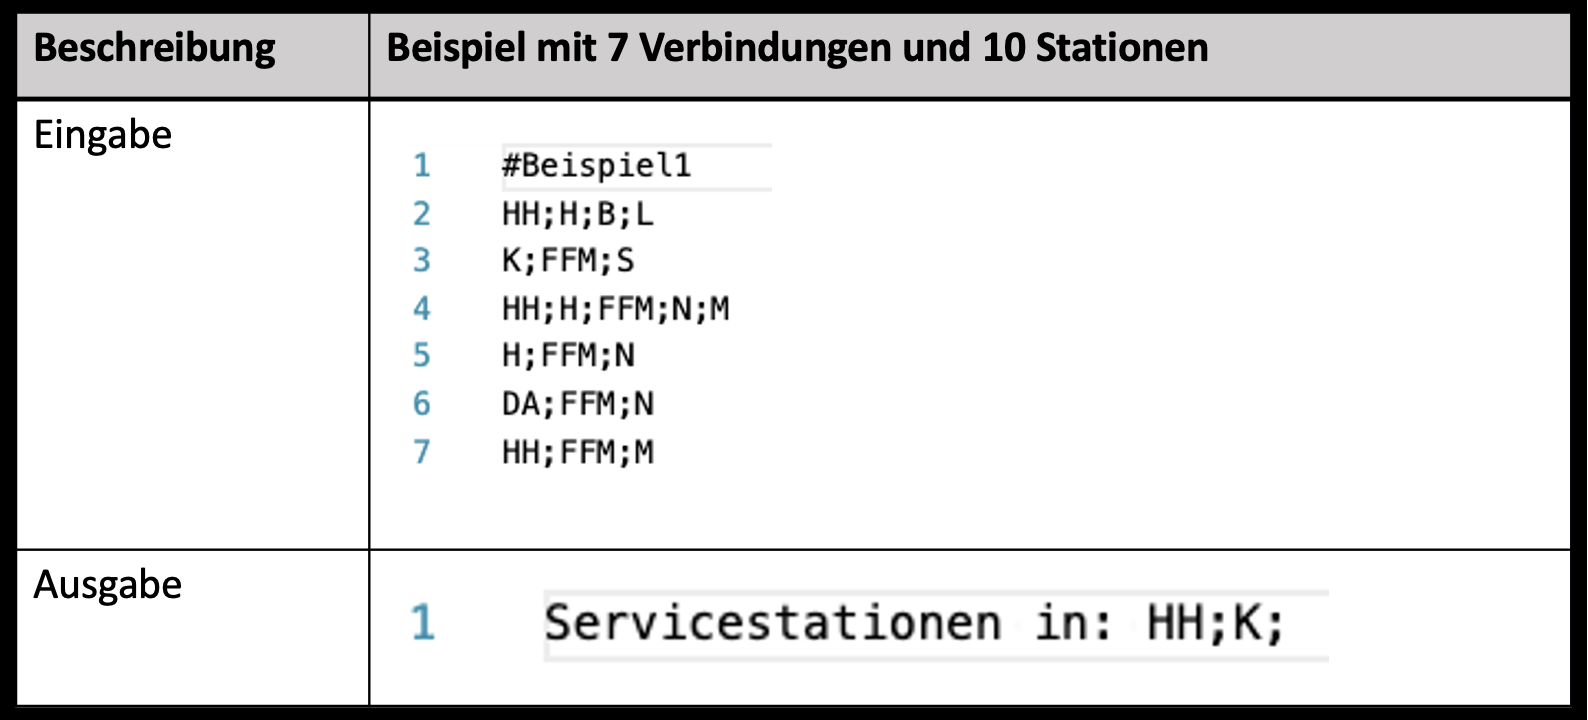
\includegraphics[width=\linewidth]{images/Tests/IHK-Beispiele/Beispiel1.png}
    \label{test:subsecpar:beispiel1}
\end{center}

\begin{center}
    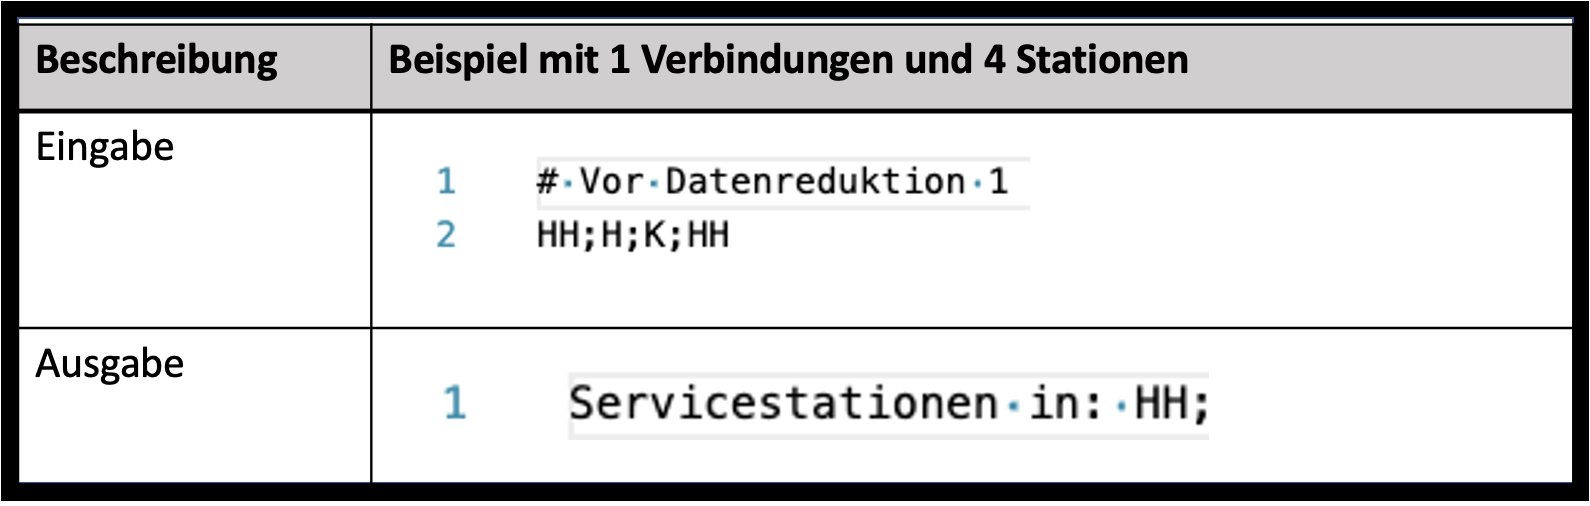
\includegraphics[width=\linewidth]{images/Tests/IHK-Beispiele/Datenreduktion1.png}
    \label{test:subsecpar:Datenreduktion1}
\end{center}

\begin{center}
    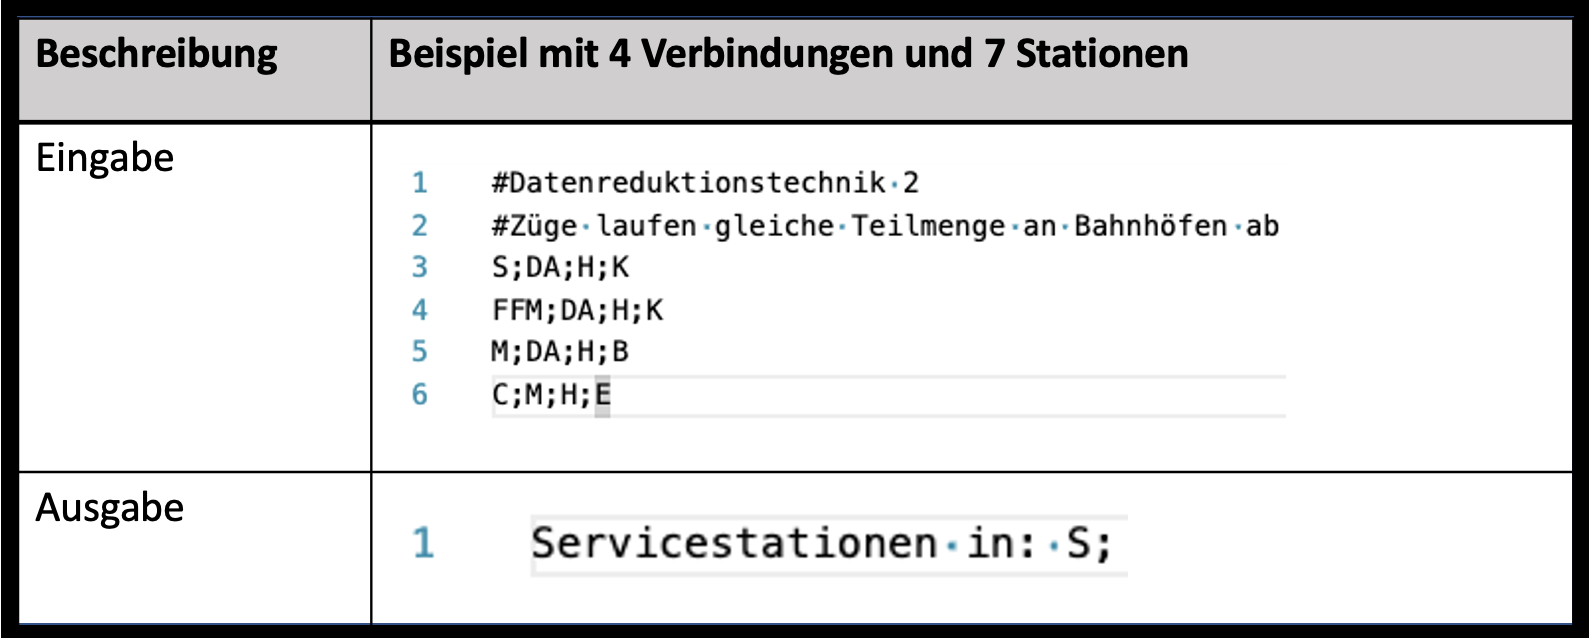
\includegraphics[width=\linewidth]{images/Tests/IHK-Beispiele/Datenreduktion2.png}
    \label{test:subsecpar:Datenreduktion2}
\end{center}

\begin{center}
    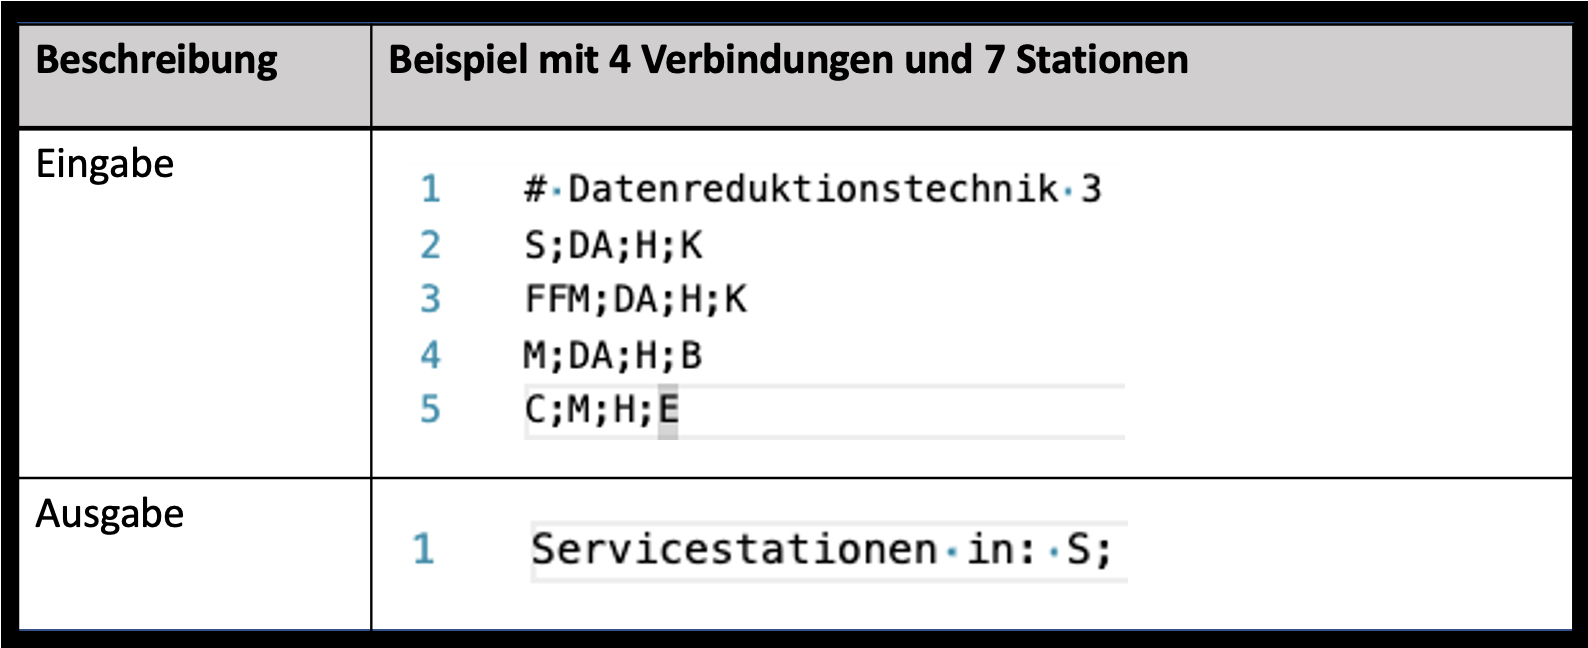
\includegraphics[width=\linewidth]{images/Tests/IHK-Beispiele/Datenreduktion3.png}
    \label{test:subsecpar:Datenreduktion3}
\end{center}


\subsection{Fehlerfälle}\label{test:sec:fehlerfaelle}
Die folgenden Test decken die in \ref{auf:sec:fehlerarten} gennanten Fehlerfälle ab.

\subsubsection{Technische Fehler}\label{test:sec:technische-fehler}
\begin{center}
    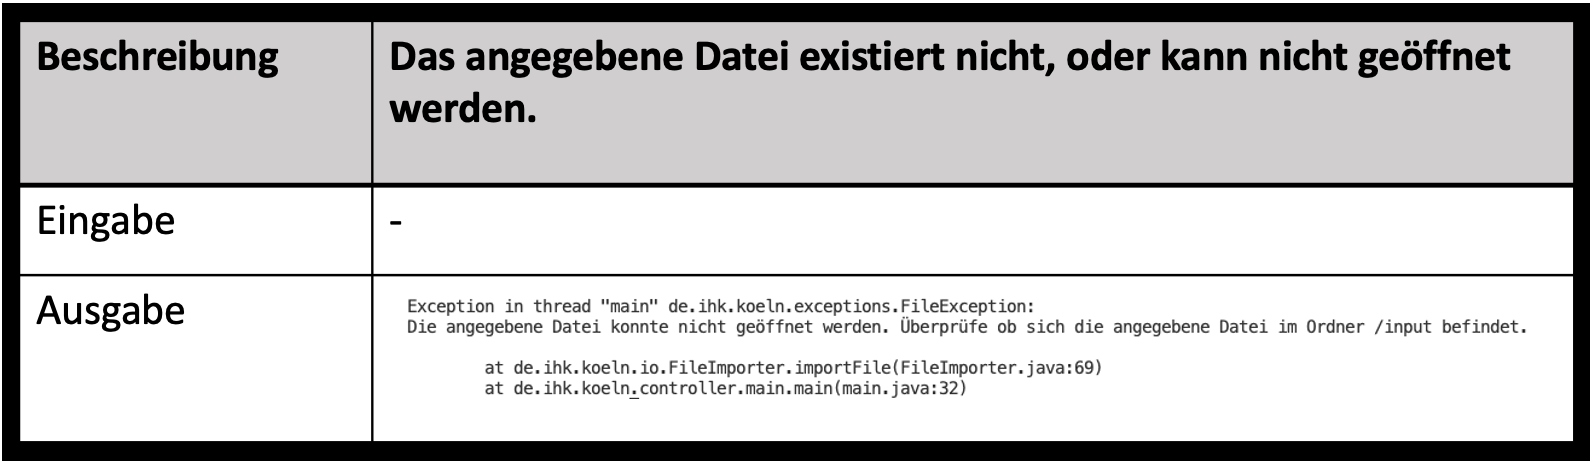
\includegraphics[width=\linewidth]{images/Tests/Fehlerfälle/FileException.png}
    \label{test:subsecpar:einlese-fehler}
\end{center}

\begin{center}
    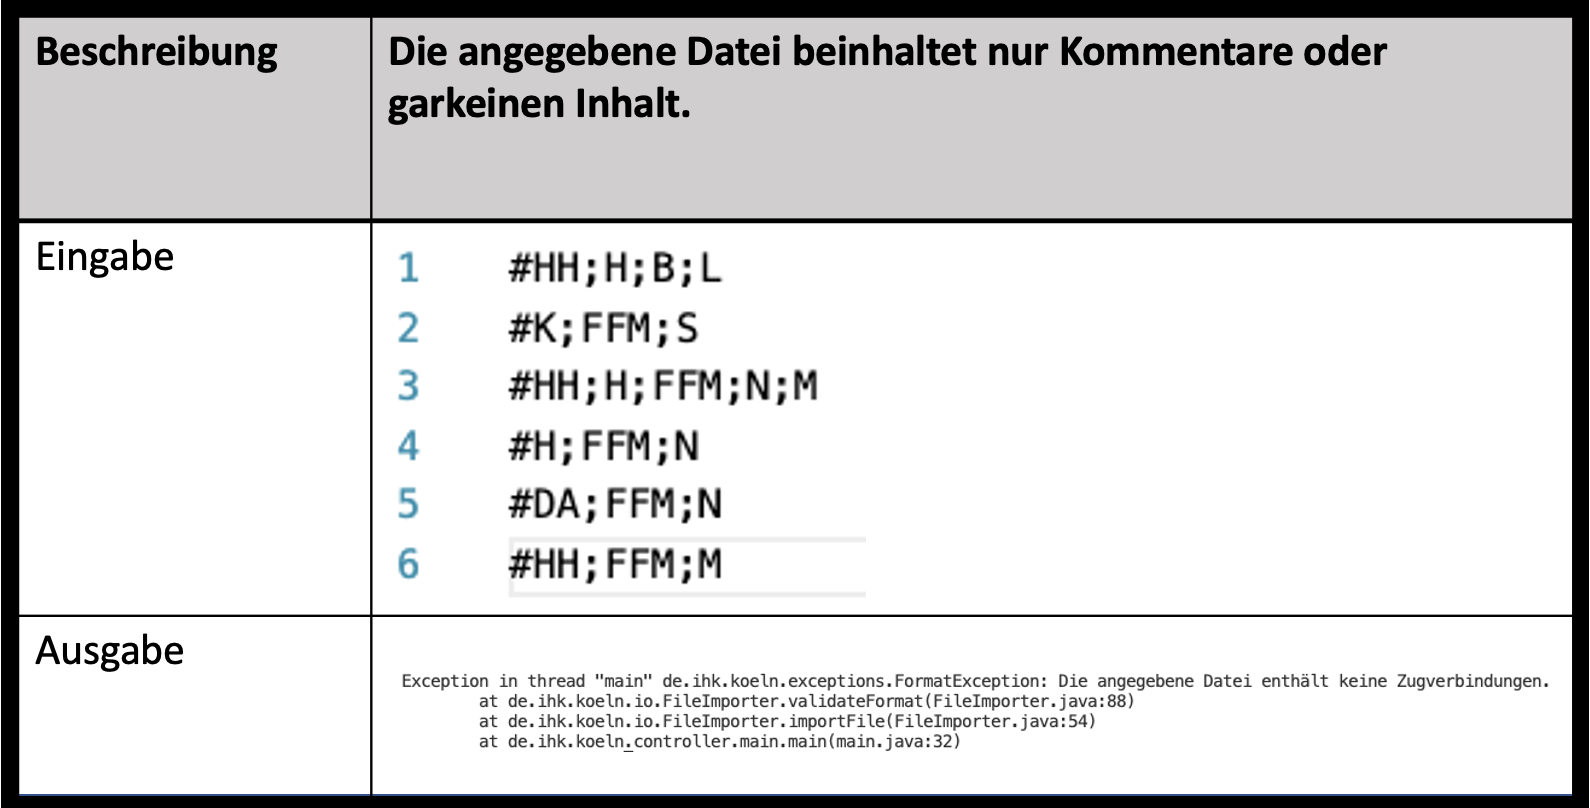
\includegraphics[width=\linewidth]{images/Tests/Fehlerfälle/LerreDatei.png}
    \label{test:subsecpar:leere-datei}
\end{center}

\subsubsection{Syntaktische Fehler}\label{test:sec:syntaktische-fehler}
\begin{center}
    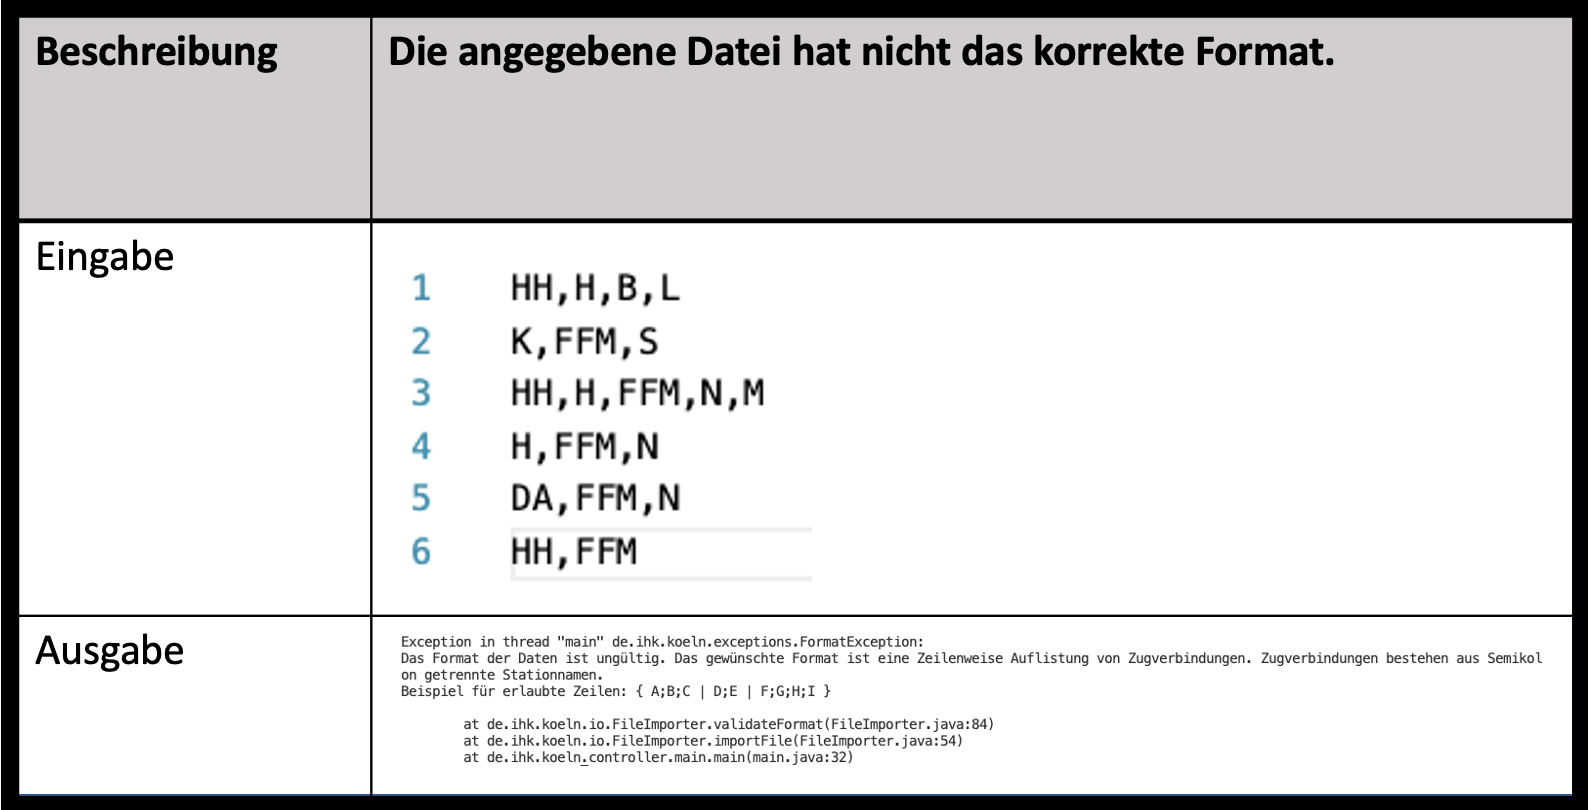
\includegraphics[width=\linewidth]{images/Tests/Fehlerfälle/FormatException.png}
    \label{test:subsecpar:format-fehler}
\end{center}

\subsubsection{Semantische Fehler}\label{test:sec:semantische-fehler}
\begin{center}
    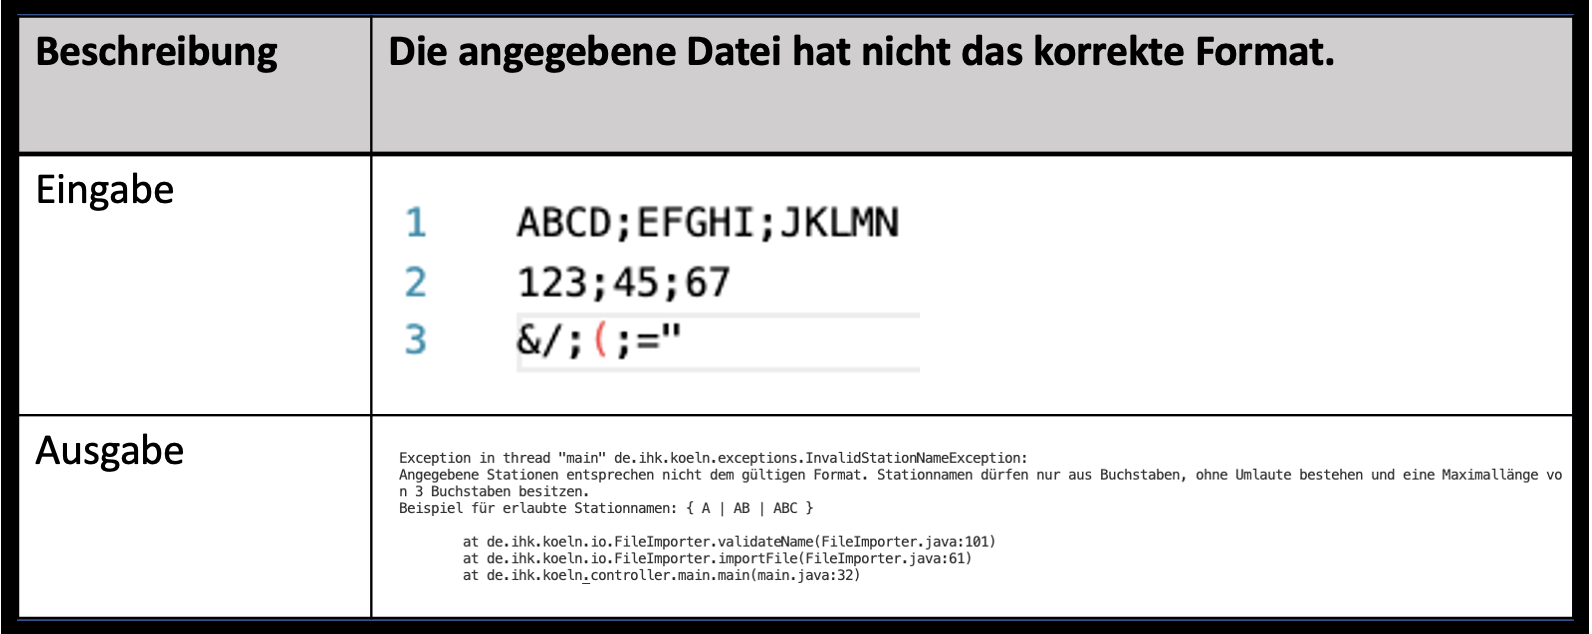
\includegraphics[width=\linewidth]{images/Tests/Fehlerfälle/InvalidNameException.png}
    \label{test:subsecpar:namen-sind-nicht-erlaubt}
\end{center}

\subsection{Grenzfälle}\label{test:sec:grenzfaelle}

\begin{center}
    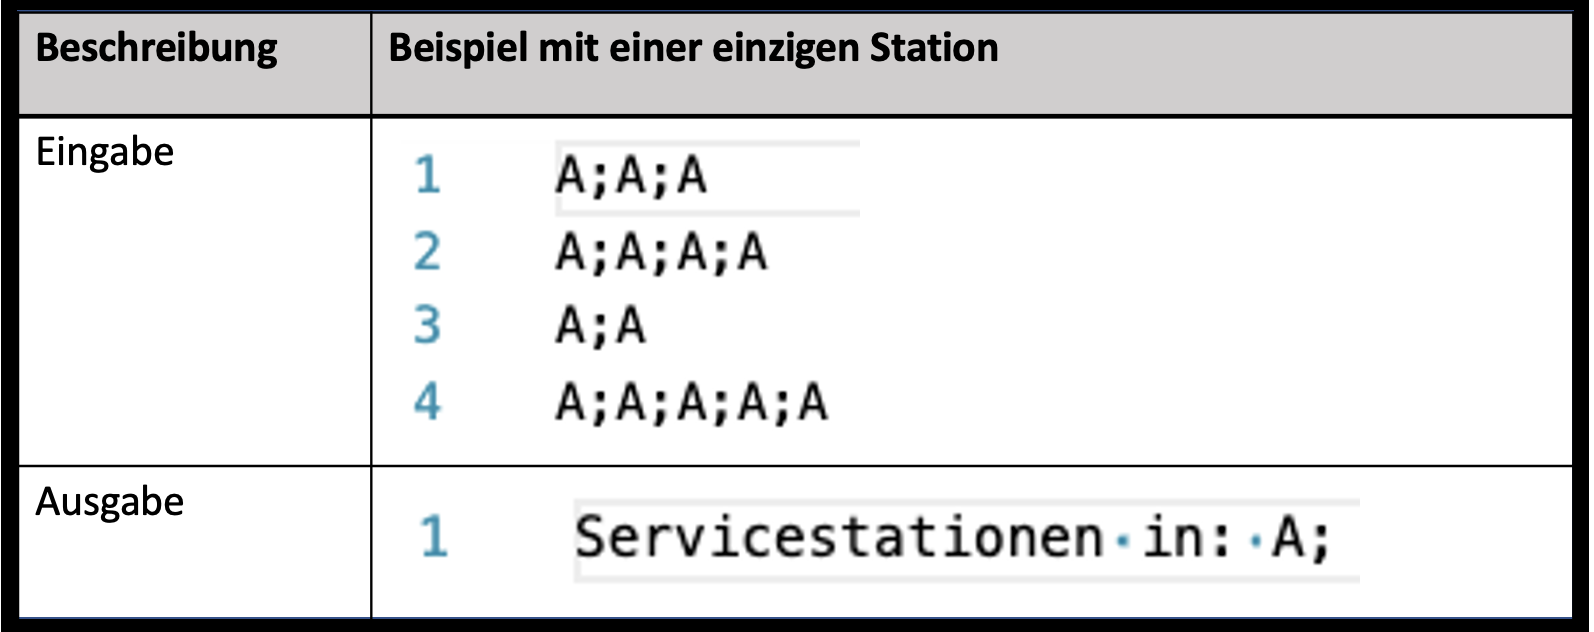
\includegraphics[width=\linewidth]{images/Tests/Grenzfälle/einzigeStation.png}
    \label{test:subsecpar:einzige-station}
\end{center}

\begin{center}
    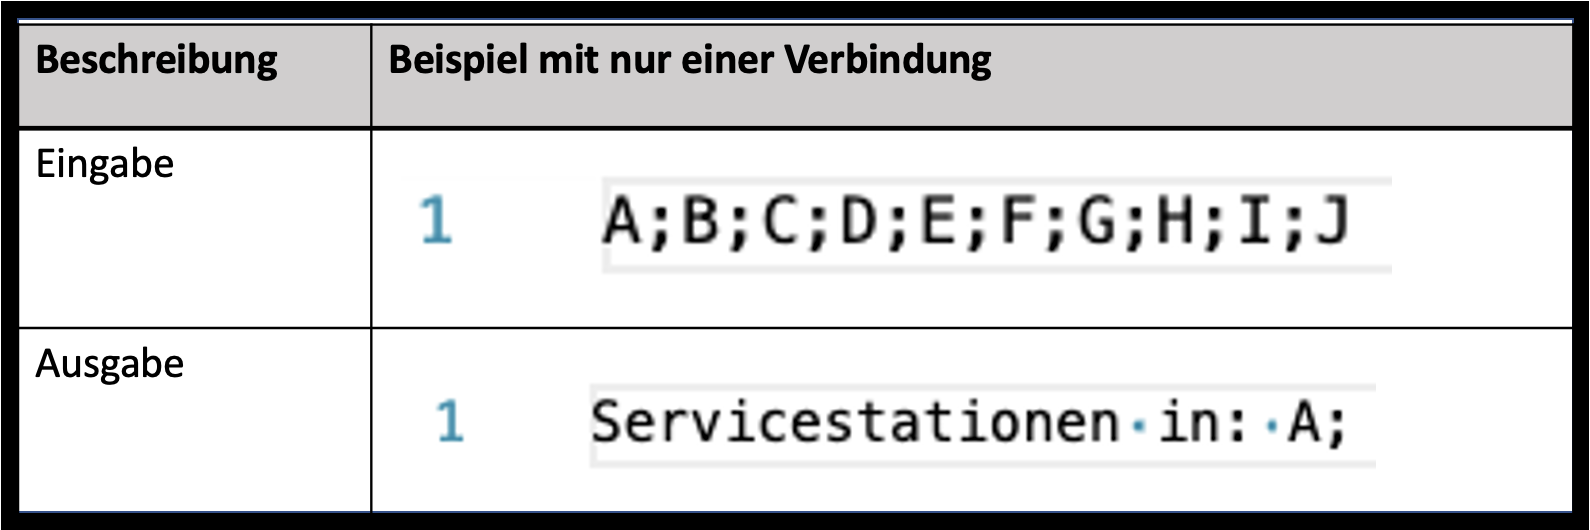
\includegraphics[width=\linewidth]{images/Tests/Grenzfälle/einzigeVerbindung.png}
    \label{test:subsecpar:einzige}
\end{center}


\subsection{Sonderfälle}\label{test:sec:sonderfaelle}

\begin{center}
    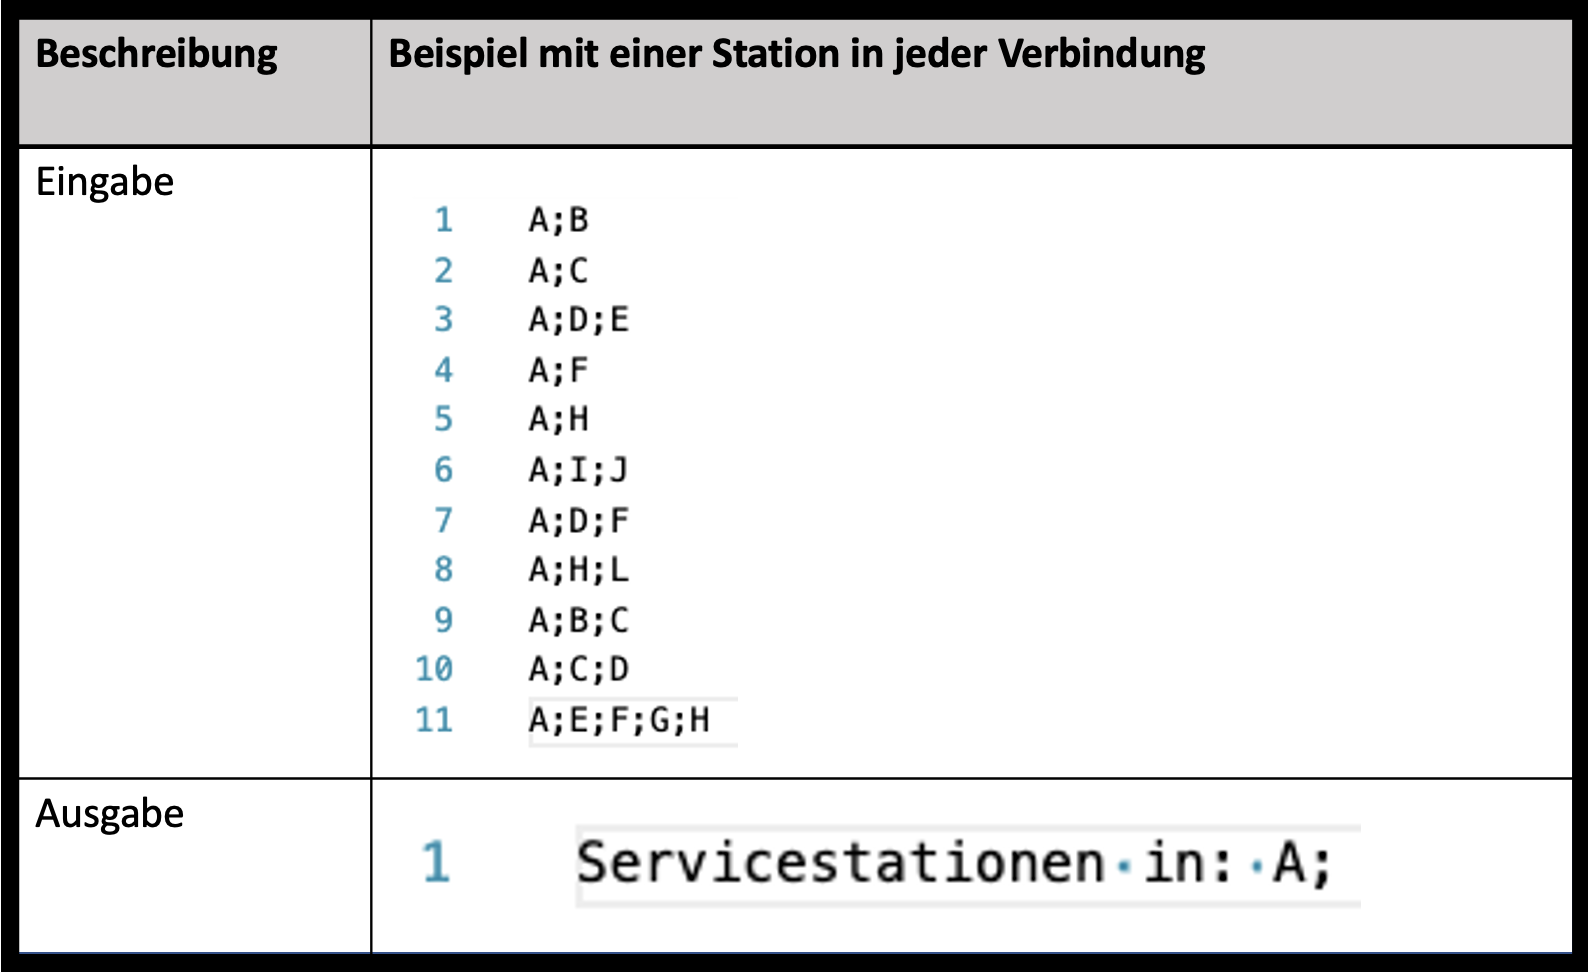
\includegraphics[width=\linewidth]{images/Tests/Sonderfälle/uerbergreifendeStation.png}
    \label{test:subsecpar:uerbergreifendeStation}
\end{center}

\begin{center}
    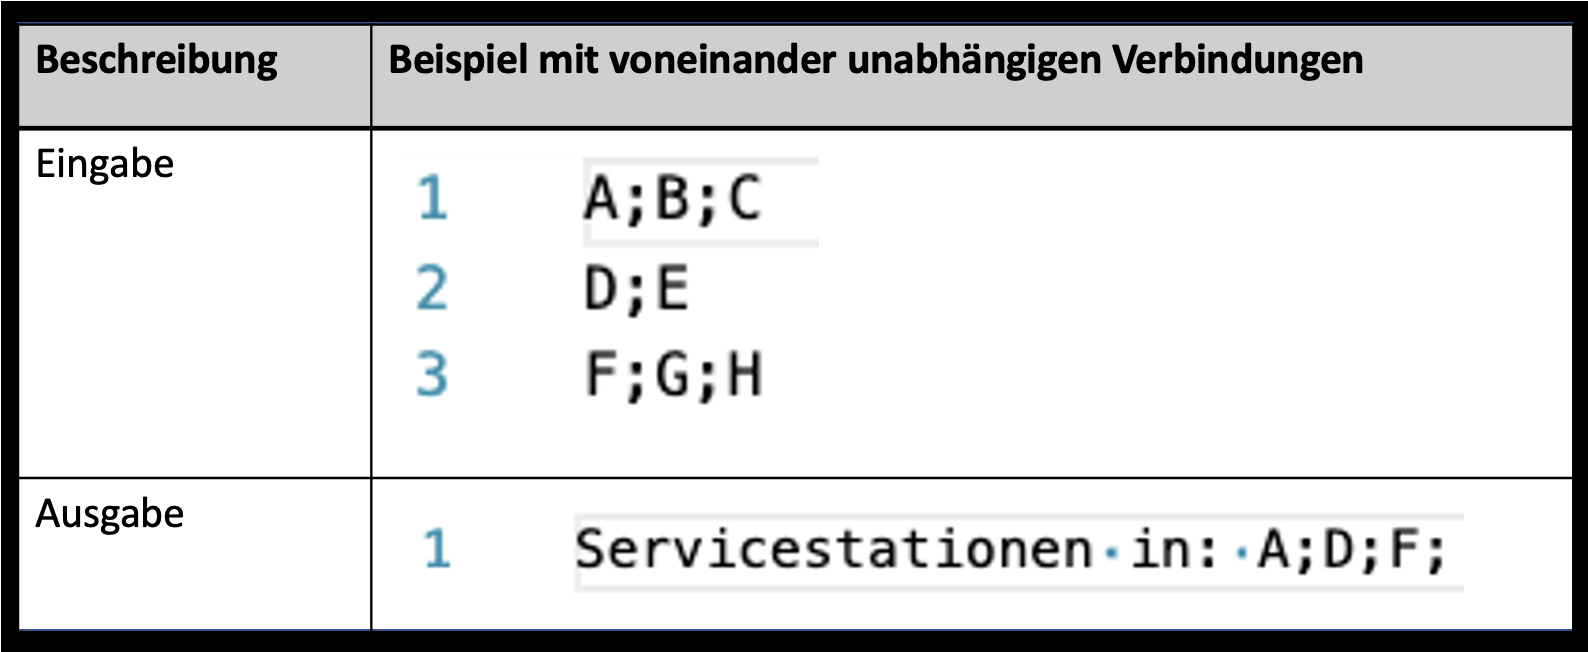
\includegraphics[width=\linewidth]{images/Tests/Sonderfälle/unabhaengigeStationen.png}
    \label{test:subsecpar:unabhaengigeStationen}
\end{center}


\section{Ausführliches Beispiel}\label{test:sec:ausfuehrliches-beispiel}
Im folgendem wird für ein Bahnnetz ein kompletter Programmdurchlauf beschrieben.\\

Dafür wird folgende Datei eingelesen:\\
\begin{center}
    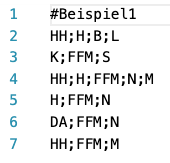
\includegraphics[scale=0.75]{images/Programmdurchlauf/eingabedatei.png}
    \label{test:subsecpar:eingabedatei}
    \captionof{figure}{Eingabedatei}
\end{center}

Beim lesen der Datei werden Kommentare ignoriert und die Zeilen in Zugverbindungen umgewandelt. Dabei wird auf korrekte Syntax geachtet.
Sind alle Verbindungen eingelesen werden die Stationen ermittel. Zusammen werden diese in einem Zugnetz gespeichert. Das vorliegende Zugnetz liegt folgendermaßen vor:\\

\begin{center}
    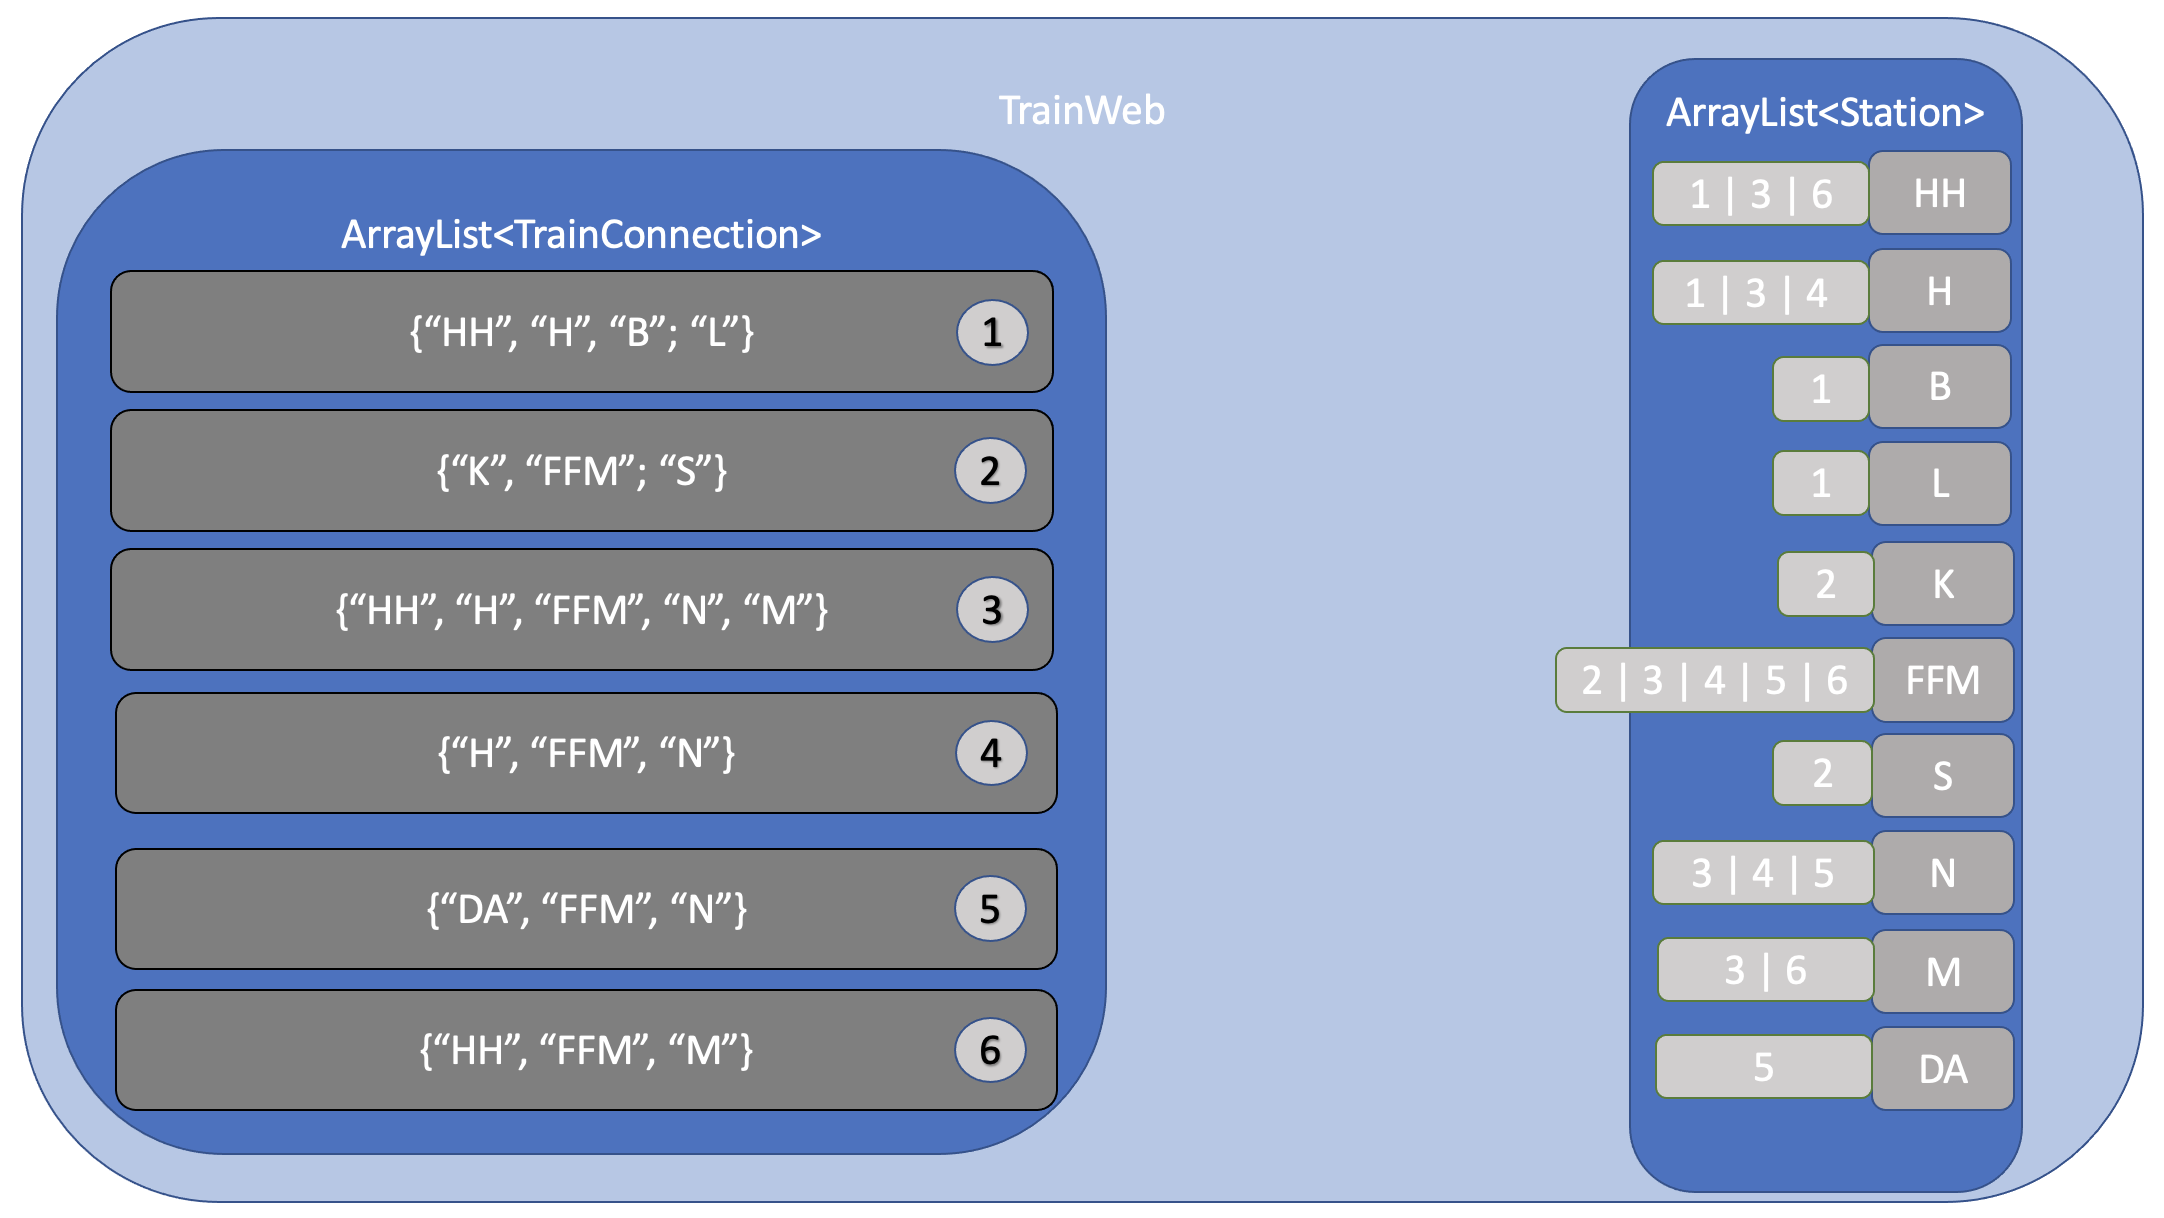
\includegraphics[width=\linewidth]{images/Programmdurchlauf/Datenstruktur01.png}
    \label{test:subsecpar:datenstruktur1}
    \captionof{figure}{Datenstruktur}
\end{center}

Diese Zugnetz wird nun Reduziert. Dafür werden die drei Reduktionsverfahren angewandt.\\
Die erste Reduktiontechnik überprüft ob eine Station mehrfach in einer Zugverbindung vorkommt. Ist dies der Fall werden alle doppelten vorkommen entfernt.\\
Da in diesem Fall keine doppelten Stationen vorkommen, wird das Netz nicht verändert.
\begin{center}
    \textit{siehe \ref{test:subsecpar:datenstruktur1}}
\end{center}

Die zweite Reduktionstechnik fasst Stationen zusammen, die keinen Aussagewert haben. Dies ist dann der Fall, wenn jede Verbindung die Station A anfährt auch eine Station B beinhaltet. In diesem Fall kann Station A gelöscht werden.\\
Stationen \texttt{K}, \texttt{S}, \texttt{B}, \texttt{L} und \texttt{DA} tauchen in jeweils nur einer Verbindung vor. Solang diese noch weiter Stationen beinhalten können diese sofort entfernt werden. Betrachtet man Station \texttt{M} und \texttt{N} lässt sich feststellen, dass diese in allen Verbindungen auch \texttt{FFM} anfahren und somit ebenfalls entfernt werden können.\\
Das Bahnnetz liegt nun folgendermaßen vor:\\

\begin{center}
    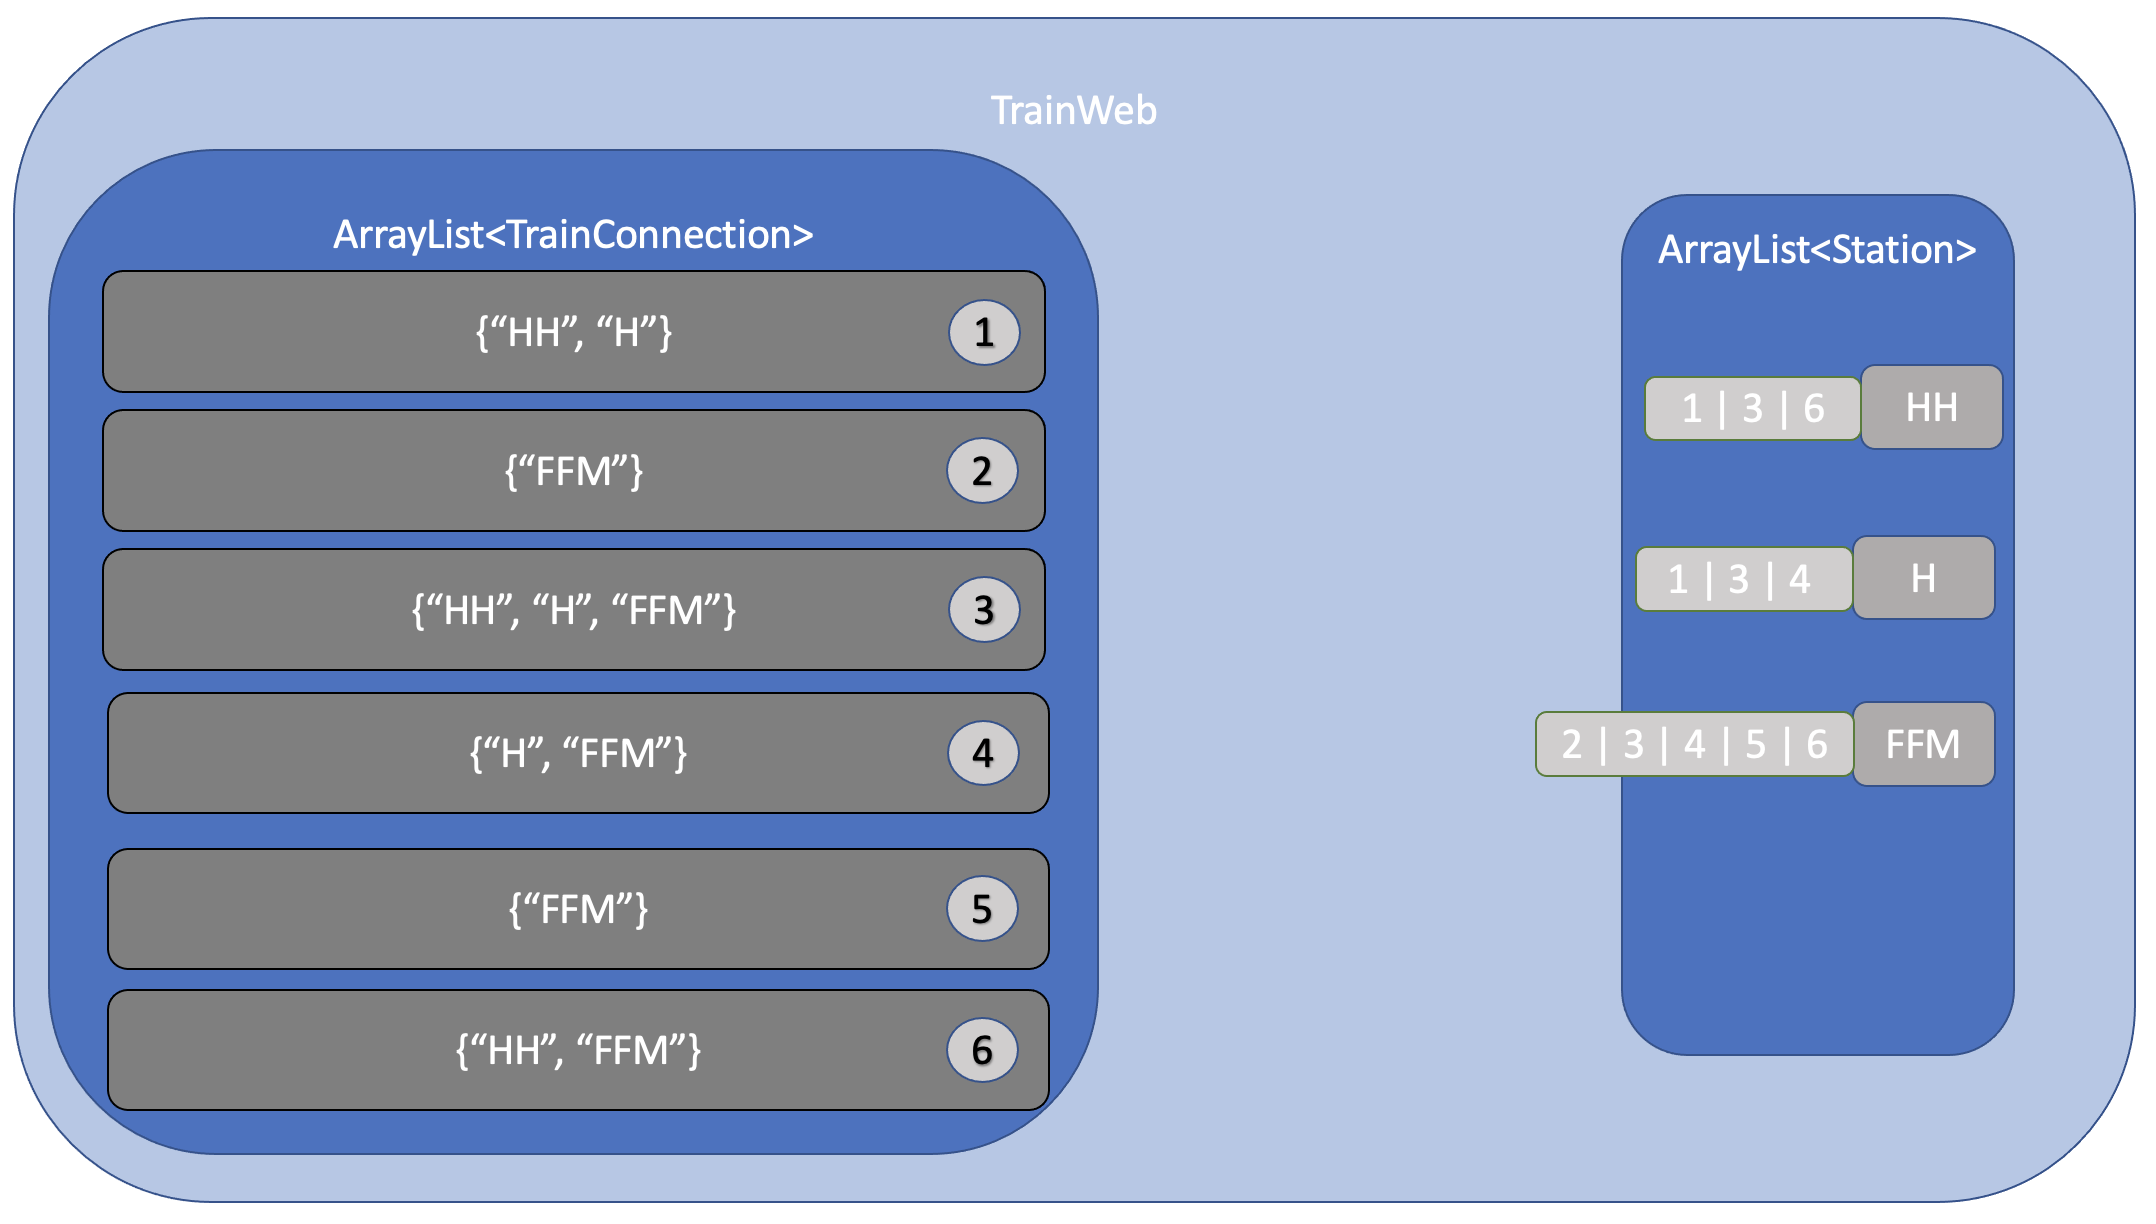
\includegraphics[width=\linewidth]{images/Programmdurchlauf/Datenstruktur02.png}
    \label{test:subsecpar:datenstruktur2}
    \captionof{figure}{Ergebnis der zweiten Datenreduktion}
\end{center}

Die dritte Reduktionstechnik überprüft ob eine Zugverbindung implizit in einer anderen Zugverbindung enthalten ist. Ist dies der Fall kann die größere Zugverbindung entfernt werden. Das gilt auch für Verbindungen die die genau selben Stationen anfahren.\\
Dafür werden die Verbindungen mit den wenigsten Stationen betrachtet. In diesem Fall bestehen Verbindung 2 und 5 nurnoch aus der Station \texttt{FFM}. Verbindungen, welche die Teilstrecke \texttt{FFM} beinhalten können nun entfernt werden. Das heißt auch, das Verbindungen die equivalent zur betrachteten Verbindung ist, also die exakt selben Stationen anfährt, ebenfalls entfernt werden kann.\\
Die übergebliebenen Verbindungen ergeben folgendes Bahnnetz:\\

\begin{center}
    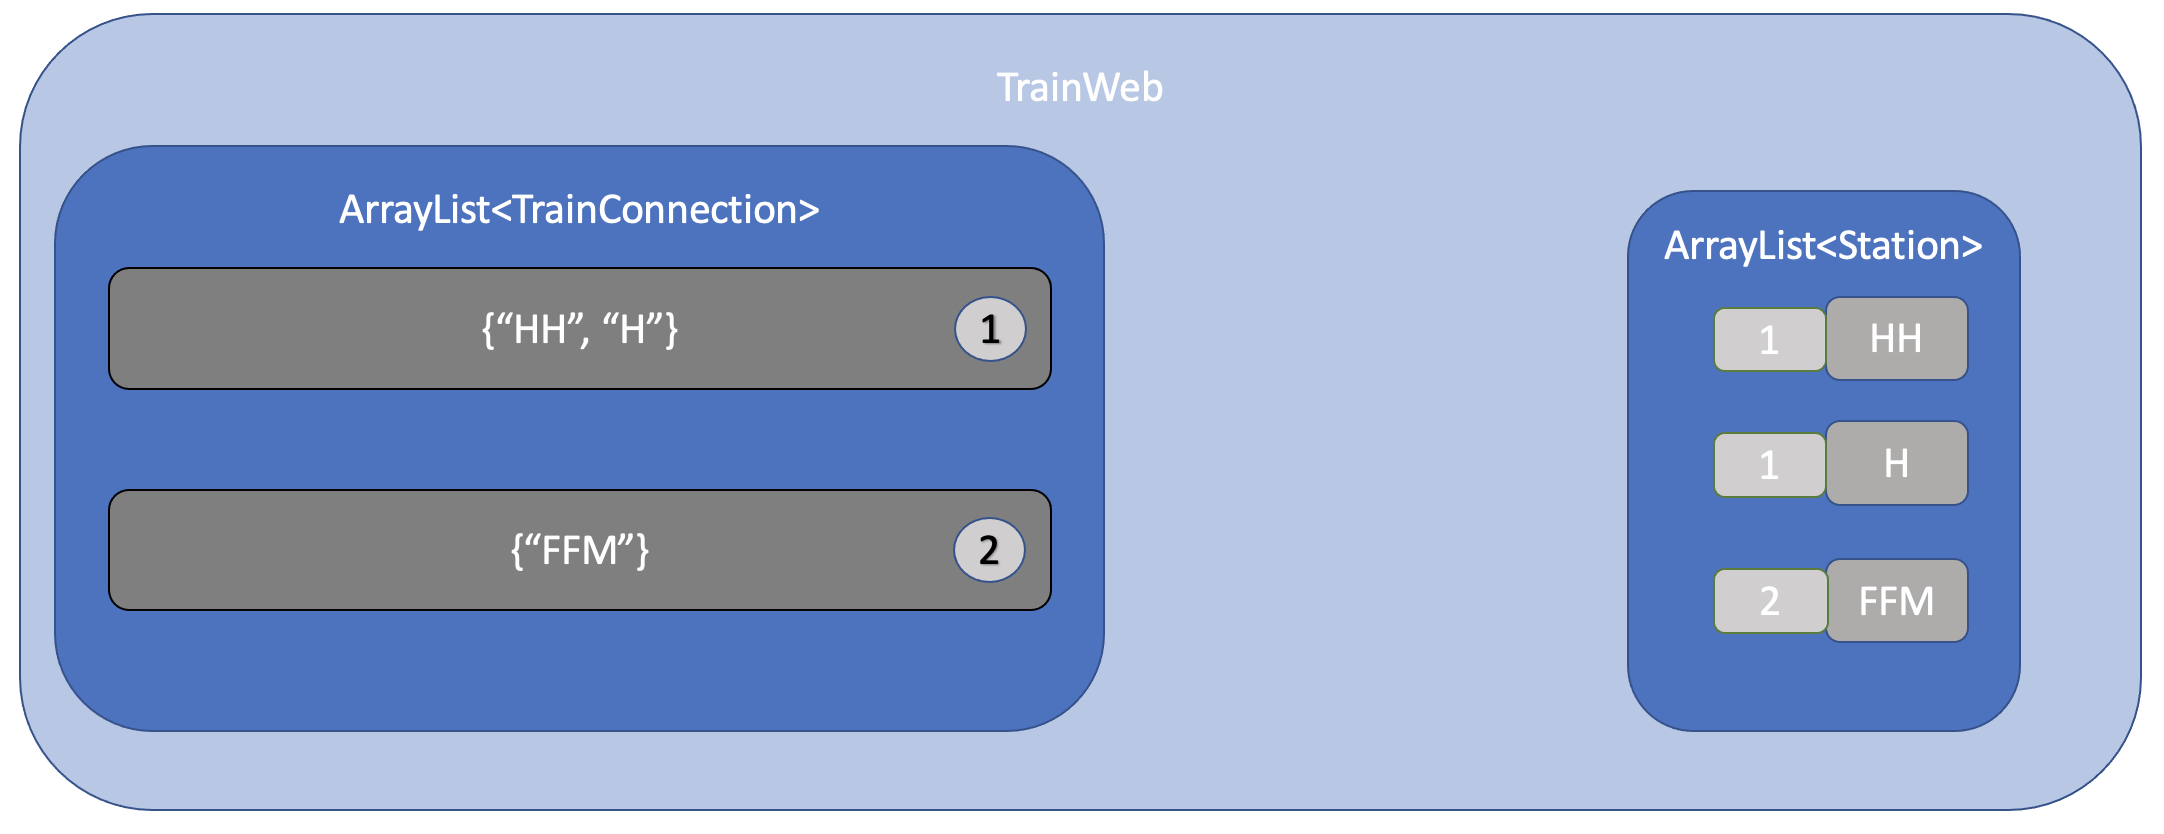
\includegraphics[width=\linewidth]{images/Programmdurchlauf/Datenstruktur03.png}
    \label{test:subsecpar:datenstruktur3}
    \captionof{figure}{Ergebnis der dritten Datenreduktion}
\end{center}

Das nun reduzierte Bahnnetz kann jetzt dem Algorithmus übergeben werden, welcher die Stationen ausgewählt, die als Servicestation verwerndet werden können.\\
Dafür wir die Station ausgewählt, die in den meisten Verbindungen vorkommt. In diesem Fall haben alle Stationen gleich viele Verbindungen sodass eine beliebige Station gewählt werden kann. Diese Station wird in eine Liste von Stationen gegeben.\\

\begin{center}
    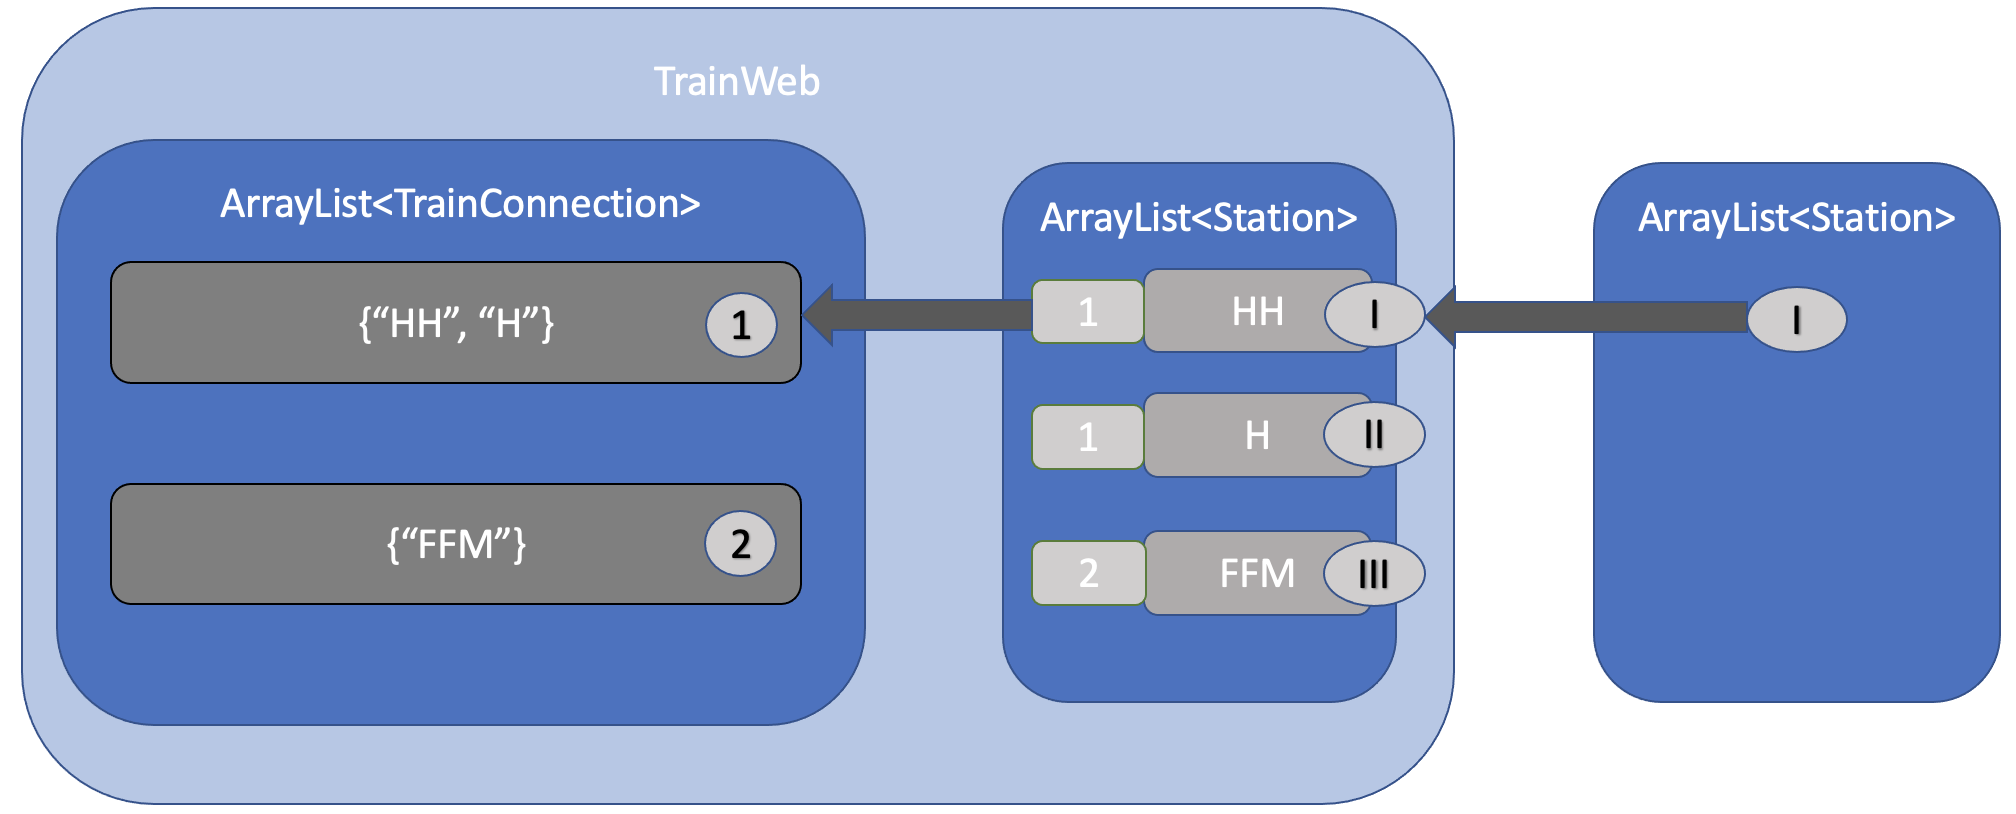
\includegraphics[width=\linewidth]{images/Programmdurchlauf/Datenstruktur04.png}
    \label{test:subsecpar:datenstruktur04}
    \captionof{figure}{Algorithmus Zustand 1}
\end{center}

Nun wird verglichen, ob es noch Verbindungen gibt, die noch keine Servicestation beinhalten. Dazu werden alle Verbindungen der Stationen in der neuen Liste gesammelt und um anschluss mit allen Verbindungen des Netzplans zu verglichen.\\
Die hier hinzugefügte Station \texttt{HH} deckt die Verbindung 1 ab. Verbindung 2 ist noch nicht versorgt, sodass nun weitergesucht werden muss\\
Dafür werden alle noch nicht versorgten Verbindungen betrachtet und die Stationen ausgewählt, die in den meisten Verbindungen vorkommt.\\
Da es sich nurnoch im eine Verbindung handelt kann man eine beliebige Station der Verbindung auswählen. So kann auch \texttt{FFM} an die Liste angehängt werden.\\

\begin{center}
    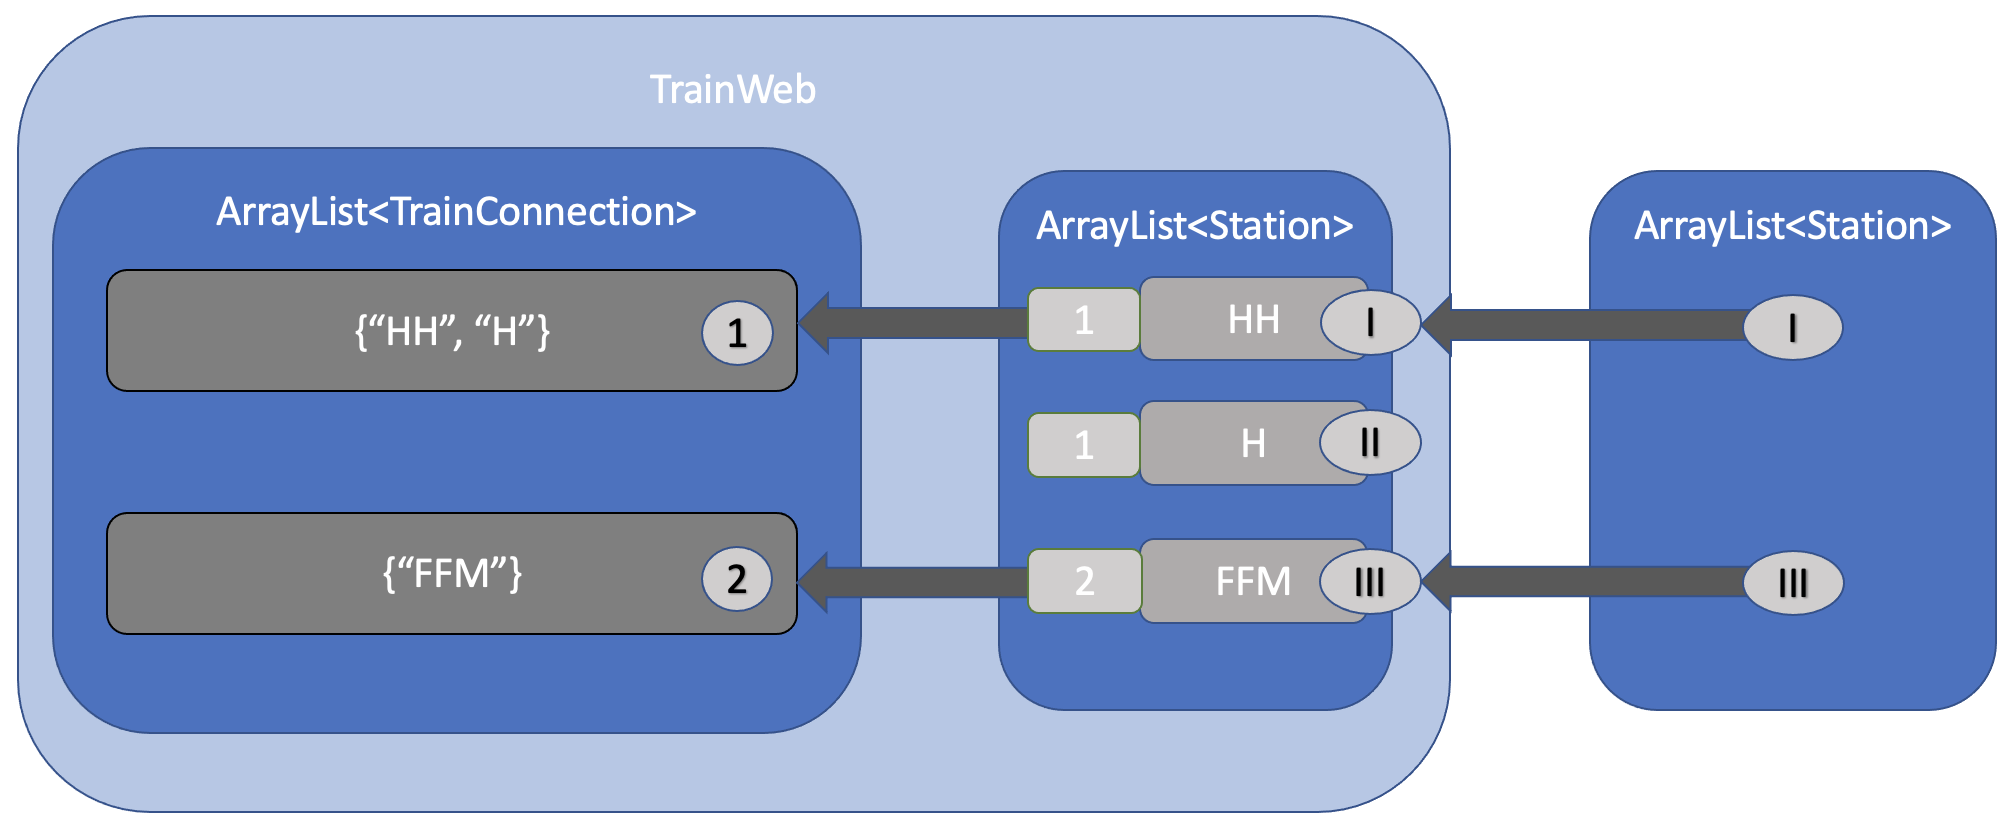
\includegraphics[width=\linewidth]{images/Programmdurchlauf/Datenstruktur05.png}
    \label{test:subsecpar:datenstruktur05}
    \captionof{figure}{Algorithmus Zustand 2}
\end{center}

Bevor überprüft werden kann, ob alle Verbindungen versorgt sind, wird jetzt überprüft, ob alle Stationen der Liste wirklich gebraucht werden.\\
Dazu wird verglichen ob die komplette Liste die selben Verbindungen abdecken kann wie die Liste ohne eine Station. Sollte dies der Fall sein, wird die Station aus der Liste entfernt. Wurden mehere Stationen gefunden werden, wird die Station gelöscht, die in mehr Verbindungen vorkommt entfernt. Konnte eine Station gelöscht werden wiederholt sich der Kontrollprozess solange, wie noch Stationen gefunden werden, die entfernt werden können.\\
In diesem Fall gibt es jedoch keine Verbindung, die gelöscht werden kann.\\

Jetzt kann überprüft werden, ob alle Verbindungen versorgt sind. In diesem Fall beinhalten alle Verbindungen mindestens eine Station der neuen Liste.\\
Somit ist die Liste der Servicestationen vollständig und kann ausgegeben werden.\\

Dafür wird folgendes Dokument ausgegeben:\\
\begin{center}
    
\includegraphics[width=\linewidth]{images/Programmdurchlauf/ausgabedatei.png}
    \label{test:subsecpar:ausgabedatei}
    \captionof{figure}{Ausgabedatei}
\end{center}

Der Programmdurchlauf ist nun abgeschlossen.\\